\documentclass[dvipdfmx]{jsarticle}
\usepackage[dvipdfmx]{graphicx}
\usepackage{amsmath, amssymb}
\usepackage{mathtools}
\usepackage{here}

\renewcommand{\thefigure}{\thesection-\arabic{figure}}
\setcounter{section}{5}
\setcounter{figure}{5}

\begin{document}
\section*{5.2 連鎖律}
計算グラフの順伝播は,計算結果を左から右へ伝達するものだった.
一方,逆方向の伝播は「局所的な微分」を右から左へ伝達するものである.
この「局所的な微分」を伝達する原理は,\textbf{連鎖律}(chain rule)によるものである.


\section*{5.2.1 計算グラフの逆伝播}
早速,$y = f(x)$という計算があるとして,この計算の逆伝播を図5-6に表す.

\begin{figure}[htbp]
    \begin{center}
    
\includegraphics[width=\linewidth]{spring_lec/DL-52.png}
    \end{center}
    \caption{計算グラフの逆伝播:順方向とは逆向きに,局所的な微分を乗算する}
\end{figure}


図5-6に示すように,逆伝播の計算は信号$E$に対し,ノードの局所的な微分$(\partial y/\partial x)$を乗算し,それを次のノードに伝達していく.局所的な微分とは,$y = f(x)$の微分を求めるということである.
このような計算手順を踏むことでで,逆伝播は目的とする微分の値を効率よく求められる.これには,連鎖律が関係している.

\section*{5.2.2 連鎖律とは}
連鎖律の説明には,まず\textbf{合成関数}を説明する必要がある.
合成関数とは複数の関数によって構成される関数のことである.
例えば,$z = (x + y)^2$という式は,次の式(5.1)のように,2つの式で構成される.

\begin{align*}
z &= t^2 \\
t &= x + y
\tag{5.1}
\end{align*}

そして,連鎖律とは合成関数の微分が,合成関数を構成する各関数の微分の積によって表される性質のことである.
式(5.1)の例で言えば,$\partial z/ \partial x$は$\partial z/ \partial t$と$\partial t/ \partial x$の積によって表すことができる.
数式では,式(5.2)のように書ける.
\begin{equation}
    \frac{\partial z}{\partial x} = \frac{\partial z}{\partial t} \frac{\partial t}{\partial x}
\tag{5.2}
\end{equation}

\section*{5.2.3 連鎖律と計算グラフ}
では,式(5.1)の連鎖律を用いた微分を,計算グラフで表してみる.2乗の計算を「**2」というノードで表すと,図5-7のように書ける.

\begin{figure}[htbp]
    \begin{center}
    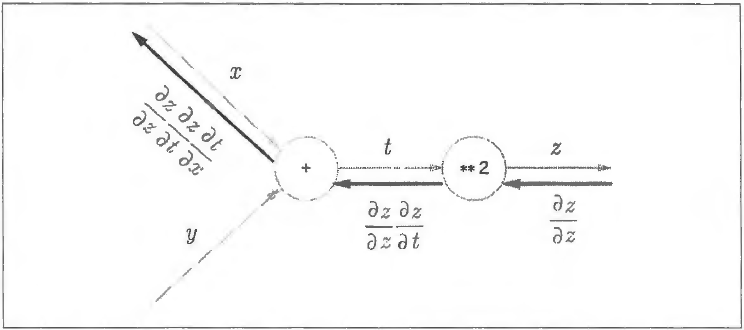
\includegraphics[width=\linewidth]{spring_lec/DL-52-2.png}
    \end{center}
    \caption{式(5.4)の計算グラフ:順方向とは逆向きの方向に,局所的な微分を乗算して渡していく}
\end{figure}

図に示したように,計算グラフの逆伝播は右から左へと信号を伝播していく.図では,「**2」への入力は$\partial z / \partial z$であり,これに局所的な微分である$\partial z / \partial t$を乗算して,次のノードへ渡していく.なお,$\partial z/ \partial z = 1$であるので,数式上は省略できる.

図5-7で注目すべきは,一番左の逆伝播の結果である.これは,連鎖律より,
\begin{equation*}\label{}
\frac{\partial z}{\partial z} \frac{\partial z}{\partial t} \frac{\partial t}{\partial x} = \frac{\partial z}{\partial t} \frac{\partial t}{\partial x} = \frac{\partial z}{\partial x}
\end{equation*}

\noindent
が成り立ち,「$xに関するzの微分$」に対応する.つまり,逆伝播が行っていることは,連鎖律の原理から構成されている.図5-7に計算結果を代入すると,図5-8のようになる.
\begin{figure}[htbp]
    \begin{center}
    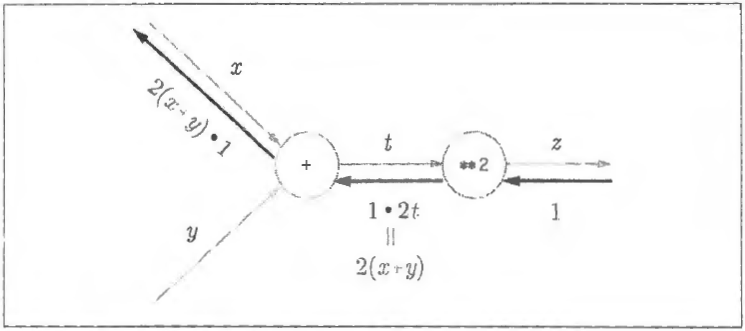
\includegraphics[width=\linewidth]{spring_lec/DL-52-3.png}
    \end{center}
    \caption{計算グラフの逆伝播の結果より,は$2(x+y)$となる}
\end{figure}

\end{document}
